\documentclass[a4j]{jsarticle}
\usepackage{graphicx}
\usepackage{listings}

\title{2024年度プログラミング\textsc{iii} 演習課題}
\author{学籍番号: 35714121 \\ 氏名: 福富隆大}
\date{2024年10月10日}
\usepackage{graphicx}

\begin{document}
\maketitle

\textbf{1 はじめに}

本レポートは演習課題第2回の実行結果をまとめたものである。

\textbf{2 課題の実行結果}

\textmd{教科書 演習2−6}

課題の実行結果を図1に示す。

\begin{figure}[htbp]
  \centering
  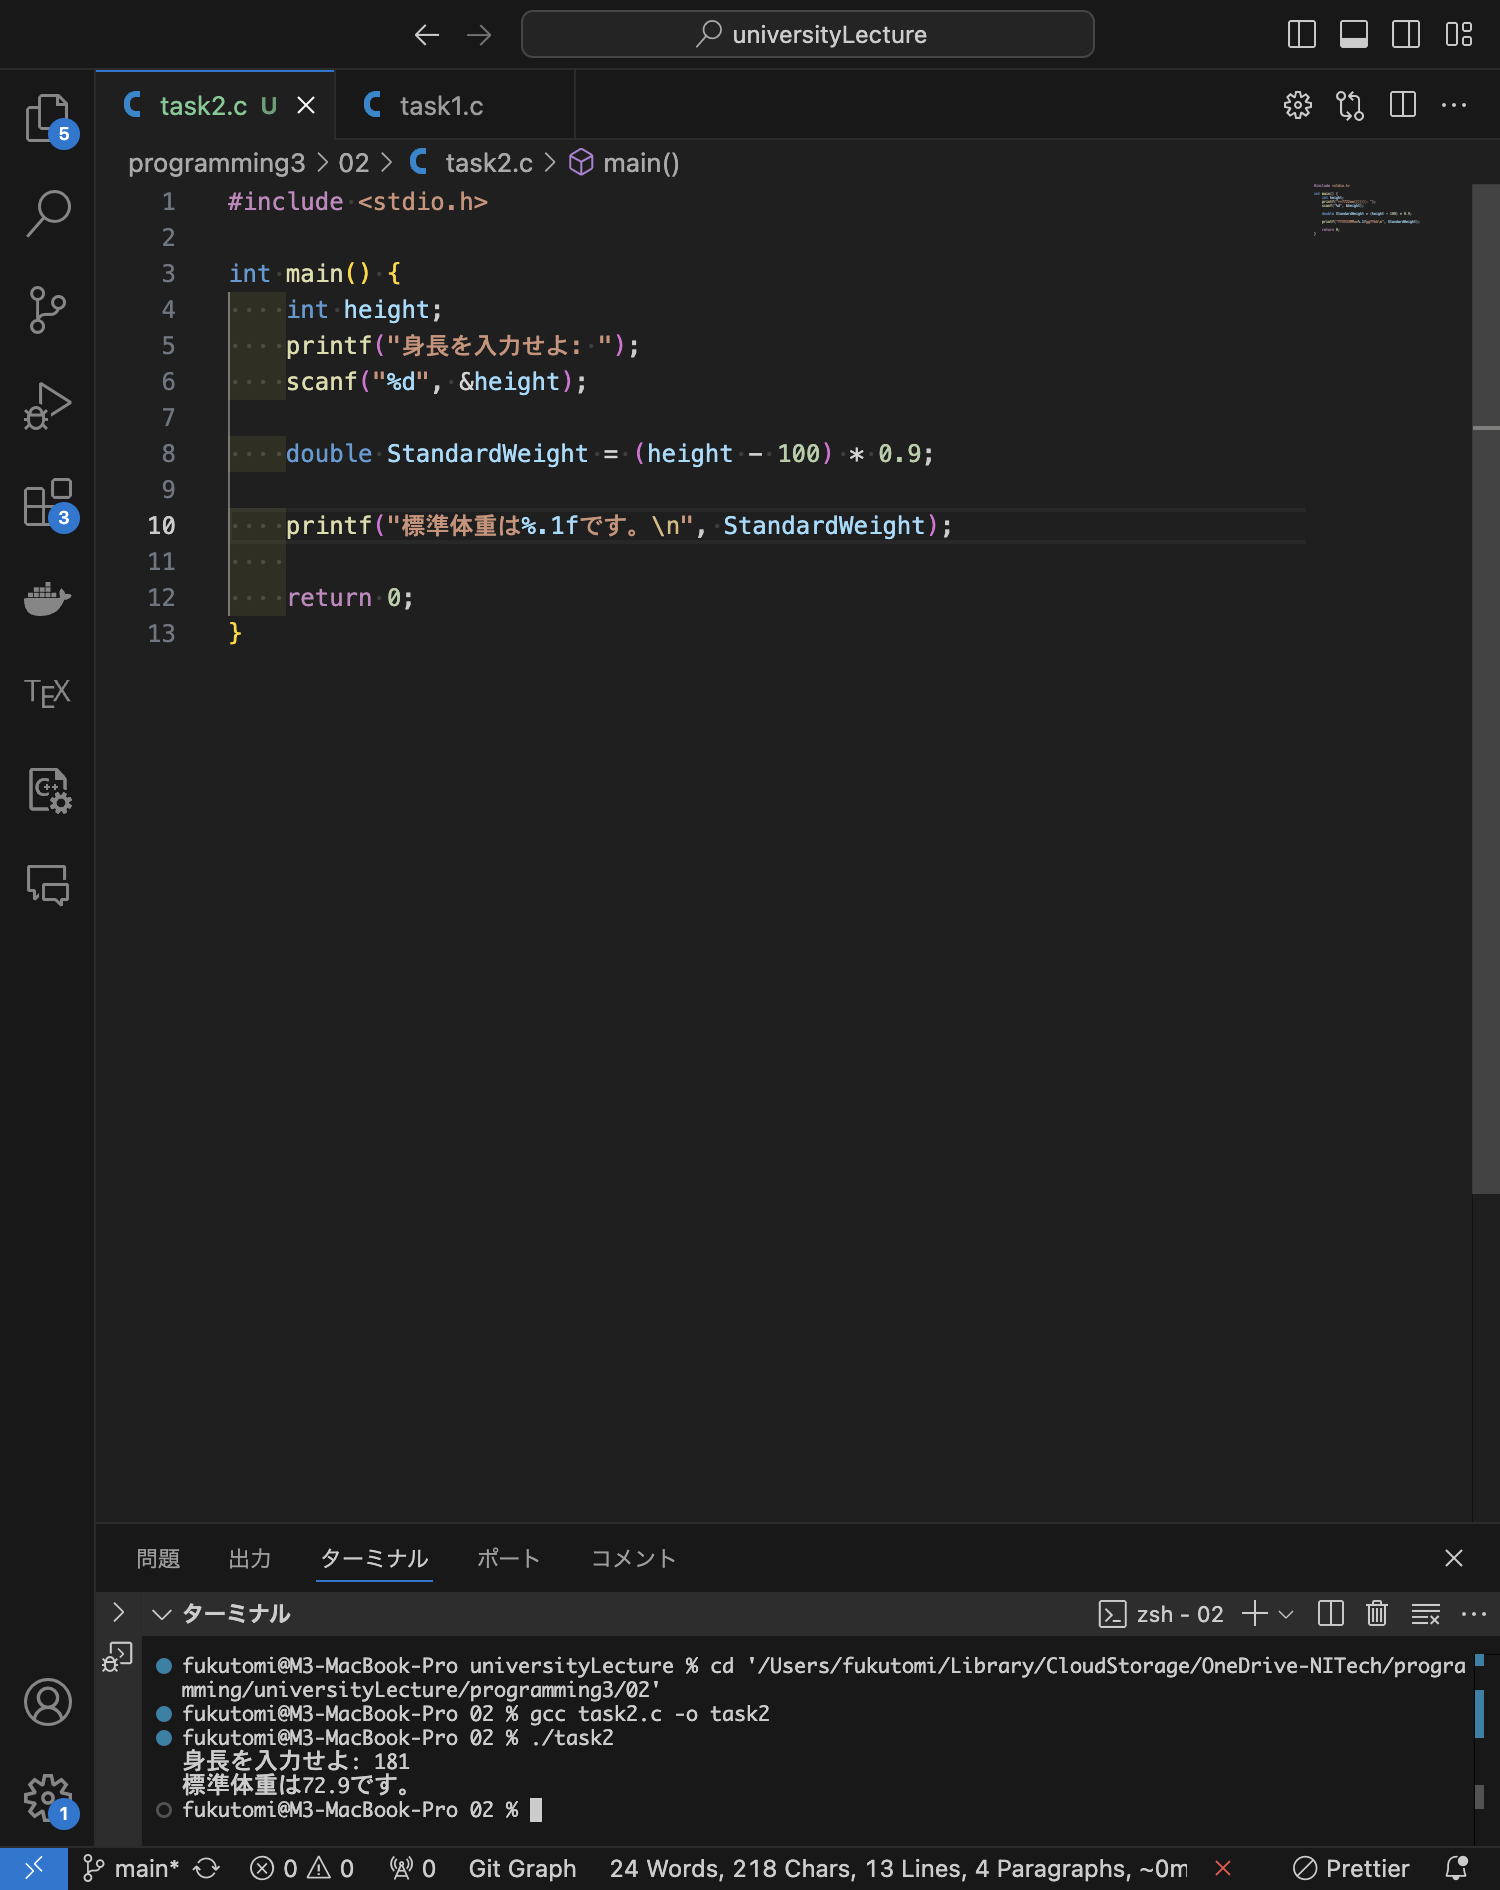
\includegraphics[width=10cm]{task2.eps}
  \caption{(画面下のターミナルの部分に実行結果があります)}
  \label{fig:sample}
\end{figure}

\textbf{3 ソースコード}

\begin{lstlisting}[language=Python, basicstyle=\ttfamily\small, frame=single]
  #include <stdio.h>

  int main() {
      int height;
      printf("身長を入力せよ: ");
      scanf("%d", &height);
  
      double StandardWeight = (height - 100) * 0.9;
  
      printf("標準体重は%.1fです。\n", StandardWeight);
      
      return 0;
  }

\end{lstlisting}

\textmd{ソースコードの説明} 

printf関数を使って「身長を入力せよ: 」と表示し、scanf関数を使って入力された身長をheightに格納する。次に、標準体重を計算し、printf関数を使って「標準体重は〇〇です。」と表示する。
小数点以下を一桁だけ表示するために、printf関数のフォーマット指定子に「.1f」を使っている。

\end{document}
